\documentclass[12pt]{standalone}

\usepackage{tikz, etoolbox}
\usetikzlibrary{arrows.meta, positioning, shapes, shapes.geometric, calc}

% Sanserif font:
\renewcommand{\familydefault}{\sfdefault}

\newcommand{\entity}[3][]{
  \node(#2)[
    entity,
    #1
  ] {
    \nodepart[font=\bfseries]{one} #2
    \nodepart{two} #3
  };
}

\tikzset{
  entity/.style = {
    draw,
    align=left,
    rectangle split,
    rectangle split parts=2,
    rectangle split ignore empty parts,
    rectangle split part align={center, left},
    minimum width=3cm,
  },
  parallellogram/.style = {
    draw,
    trapezium,
    trapezium left angle=75,
    trapezium right angle=105,
  },
  onArrow/.style = {
    fill=white,
    align=center,
  },
  has/.style = {
    -{Latex[length=3mm]},
  },
  inherits/.style = {
    -{Latex[open, length=3mm]},
  },
  bigArrow/.style = {
    -{Latex[length=5mm]},
    line width=1mm,
    font=\bfseries,
  },
  node distance=2cm and 1cm,
}

% Attempt to get a little border padding
% \usepackage[
%     left=0.20in,
%     right=0.20in,
%     top=0.20in,
%     bottom=0.20in,
% ]{geometry}


\begin{document}

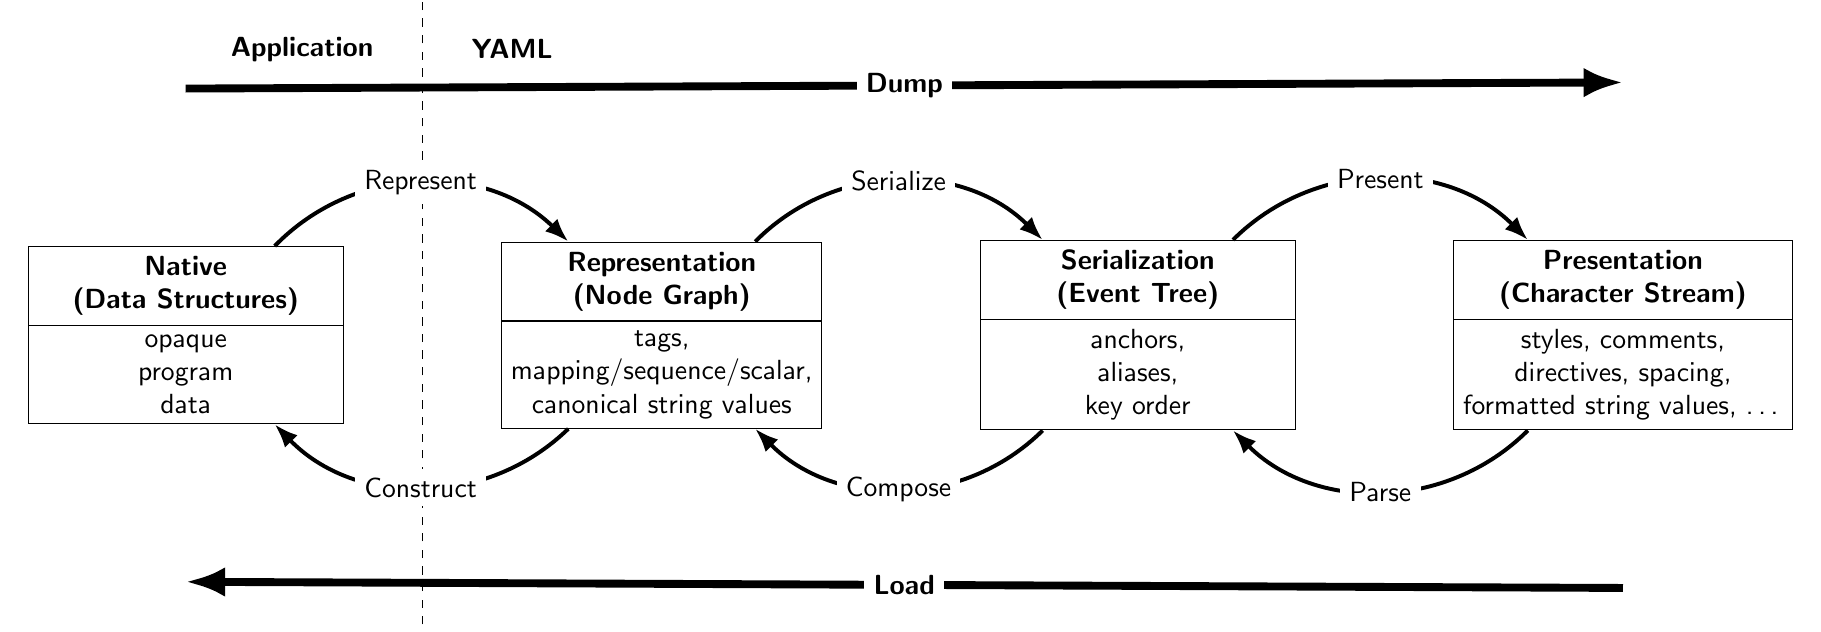
\begin{tikzpicture}[
  process/.style = {
    -{Latex[length=3mm]},
    out=45,
    in=135,
    relative,
    line width=.5mm,
  },
  stage/.style = {
    entity,
    align=center,
    rectangle split part align={center},
    minimum width=4cm,
    align=center,
  },
  node distance=2.0cm
]
\node(Native)[stage] {
  \nodepart[font=\bfseries]{one}
  Native\\(Data Structures)
  \nodepart{two}
    opaque\\
    program\\
    data
};

\node(Representation)[stage, right=of Native] {
  \nodepart[font=\bfseries]{one}
  Representation\\(Node Graph)
  \nodepart{two}
    tags,\\
    mapping/sequence/scalar,\\
    canonical string values
};

\node(Serialization)[stage, right=of Representation] {
  \nodepart[font=\bfseries]{one}
  Serialization\\(Event Tree)
  \nodepart{two}
    anchors,\\
    aliases,\\
    key order
};

\node(Presentation)[stage, right=of Serialization] {
  \nodepart[font=\bfseries]{one}
  Presentation\\(Character Stream)
  \nodepart{two}
    styles, comments,\\
    directives, spacing,\\
    formatted string values, …
};

\coordinate (Divider) at ($(Native.east)!.5!(Representation.west)$);

\draw[dashed, overlay] let \p1 = (Divider) in (\x1,-10) -- (\x1,10);

\draw
let
  \p1 = (Divider),
  \p2 = (Native.north),
  \p3 = ($(\x1,\y2)+(0,2.5)$),
in
node[left=.5cm] at (\p3) {\textbf {Application}}
node[right=.5cm] at (\p3) {\textbf {YAML}};

\draw[process] (Native) edge node[onArrow] {Represent} (Representation);
\draw[process] (Representation) edge node[onArrow] {Construct} (Native);
\draw[process] (Representation) edge node[onArrow] {Serialize} (Serialization);
\draw[process] (Serialization) edge node[onArrow] {Compose} (Representation);
\draw[process] (Serialization) edge node[onArrow] {Present} (Presentation);
\draw[process] (Presentation) edge node[onArrow] {Parse} (Serialization);

\draw[bigArrow] ($(Native.north)+(0,2)$)
  -- node[onArrow] {Dump} ($(Presentation.north)+(0,2)$);
\draw[bigArrow] ($(Presentation.south)+(0,-2)$)
  -- node[onArrow] {Load} ($(Native.south)+(0,-2)$);

\end{tikzpicture}

\end{document}
